\documentclass[british]{mscs-project}


\usepackage{tikz}
\usepackage{tikz-cd}
\usepackage{calc}
\usepackage{quiver}
\usepackage{ebproof}
\usepackage{placeins}
\usepackage{listings,newtxtt}
\usetikzlibrary{shapes,arrows}


%% Cleveref should be the last package loaded, unless you know what you are doing.
\usepackage{cleveref}


%% Define theorems after cleverref has been loeded to get the right referencing
\usepackage{thmstyle}
% Redefine Greek letters
\let\oldphi\phi
\def\phi{\varphi}
\let\oldepsilon\epsilon
\def\epsilon{\varepsilon}

% Change spacing in overset
% See https://tex.stackexchange.com/questions/194798/change-vertical-space-in-overset
\makeatletter
\newcommand{\oset}[3][0ex]{%
  \mathrel{\mathop{#3}\limits^{
    \vbox to#1{\kern-2\ex@
    \hbox{$\scriptstyle#2$}\vss}}}}
\makeatother


\newcommand*{\Q}{\mathbb{Q}}
\newcommand*{\QNN}{\Q_{\geq 0}}
\newcommand*{\QP}{\Q_{> 0}}
\newcommand*{\Z}{\mathbb{Z}}
\newcommand*{\B}{\mathbb{B}}
\newcommand*{\N}{\mathbb{N}}
\newcommand*{\Reals}{\mathbb{R}}
\newcommand*{\RNN}{\Reals_{\geq 0}}
\newcommand*{\RP}{\Reals_{> 0}}

\DeclarePairedDelimiter{\set}{\{}{\}}
\DeclarePairedDelimiterX{\setDef}[2]{\{}{\}}{#1 \; \delimsize| \; #2}
\newcommand*{\pow}{\mathcal{P}}
\DeclarePairedDelimiter{\discr}{|}{|}
\DeclarePairedDelimiter{\paren}{(}{)}
\DeclarePairedDelimiter{\braks}{[}{]}
\newcommand*{\bparen}[1]{\paren[\big]{#1}}
\DeclarePairedDelimiter{\fOrd}{[}{\rangle}

% Typeset quotients.
% Based on https://tex.stackexchange.com/questions/4624/a-symbol-for-the-quotient-of-two-objects
% and https://tex.stackexchange.com/questions/684777/include-empty-delimiter-in-declarepaireddelimiter
\NewDocumentCommand{\quot}{sO{}mm}{%
  \IfBooleanTF{#1}{% star
    \mleft.\kern-\nulldelimiterspace%
    \raisebox{.1em}{$#3$}\middle/\raisebox{-.2em}{$#4$}%
    \mright.%
  }{% no star
    \raisebox{.1em}{$#3$}#2/\raisebox{-.2em}{$#4$}%
  }%
}

\newcommand*{\from}{\colon}
\newcommand*{\natTo}{\Rightarrow}
\newcommand*{\Hom}[1]{#1}
\newcommand*{\id}{\mathrm{id}}
\newcommand*{\comp}{\circ}
\newcommand*{\op}[1]{#1^{\mathrm{op}}}
\DeclareMathOperator{\dom}{dom}
\newcommand{\proMor}[2]{%
  \begin{tikzcd}[cramped, sep=small, ampersand replacement=\&]%
    #1 \arrow[r, "\shortmid"{marking, pos=0.4}] \& #2%
  \end{tikzcd}%
}
\newcommand*{\preIm}[1]{#1^{\leftarrow}}
\newcommand*{\forIm}[1]{#1^{\rightarrow}}
\newcommand*{\preComp}[1]{#1^{\ast}}
\newcommand*{\postComp}[1]{#1_{\ast}}

\DeclarePairedDelimiter{\pair}{\langle}{\rangle}

%% Binding constructs
\newcommand*{\bind}[2]{#1 #2. \,}
\newcommand*{\all}[1]{\bind{\forall}{#1}}
\newcommand*{\exist}[1]{\bind{\exists}{#1}}
\newcommand*{\unique}[1]{\bind{\exists!}{#1}}

%%% Categories
\newcommand*{\ext}[1]{\overline{#1}}
\newcommand*{\Maps}[1]{\mathcal{#1}}
\newcommand*{\Cat}[1]{\mathcal{#1}}
\newcommand*{\CC}{\Cat{C}}
\newcommand*{\CD}{\Cat{D}}
\newcommand*{\CE}{\Cat{E}}
\DeclareMathOperator{\ob}{ob}

\DeclareMathOperator{\FunGr}{Gr}
\DeclarePairedDelimiterX{\iHom}[2]{[}{]}{#1, #2}
\newcommand*{\timesU}{\ast}
\DeclarePairedDelimiterX{\FunC}[2]{[}{]}{#1, #2}

%% Definite Categories
\newcommand*{\StdCat}[1]{\mathbf{#1}}
\newcommand*{\SetC}{\StdCat{Set}}
\newcommand*{\BSetC}{\StdCat{Set}_{\bullet}}
\newcommand*{\UBSet}{U_{\bullet}}
\newcommand*{\RelC}{\StdCat{Rel}}
\newcommand*{\Vect}{\StdCat{Vect}}
\newcommand*{\MonC}{\StdCat{Mon}}
\newcommand*{\Dom}{\StdCat{Dom}}
\newcommand*{\DDom}{\StdCat{DDiff}}
\newcommand*{\RPMod}{\RP\text{-}\StdCat{Mod}}

% Adjunctions
\newcommand*{\lTransp}[1]{#1^{\sharp}}
\newcommand*{\rTransp}[1]{#1^{\flat}}
\newcommand*{\adjointUnit}[1]{\oset[-0.3ex]{#1}{\longdashv}}
\newcommand*{\adjoint}{\dashv}
\DeclareFontFamily{U}{min}{}
\DeclareFontShape{U}{min}{m}{n}{<-> dmjhira}{}
\newcommand{\yo}{\!\text{\usefont{U}{min}{m}{n}\symbol{'107}}\:\!\!}
\newcommand{\Yo}{\!\text{\usefont{U}{min}{m}{n}\symbol{'110}}}
\newcommand{\Suba}[1]{\text{Sub}_a(#1)}
\newcommand{\Subo}[1]{\text{Sub}_0(#1)}

%% Order theory
\newcommand*{\join}{\bigvee\nolimits}
\newcommand*{\meet}{\bigwedge\nolimits}

% Geometry
% Half space with optional index for the coordinate to be tested. Default is the highest
\DeclareDocumentCommand{\Half}{o m}{%
  \mathrm{H}^{#2}\IfValueT{#1}{_{#1}}%
}

%% Convex Sets
\newcommand*{\CVec}{\StdCat{CVec}}
\newcommand*{\Conv}{\mathrm{Conv}}



\ExecuteBibliographyOptions{sorting=nyt, maxnames=99}
\addbibresource{mscs-project.bib}


% Please enter your information here
\addAuthor{Jenny Vermeltfoort}{s3787494}
\setProjectTopic{Optimisation on Analog Computers}
\setCourseYear{26-27}
\setProjectPart{II}
\setProjectUrl{\url{https://github.com/jennyvve/ms}} % Your reference has to go inside the \url command!


\begin{document}
\makeMSCSTitle{}




\tikzstyle{block} = [draw, rectangle,
   minimum height=3em, minimum width=4em]
\tikzstyle{sum} = [draw, circle, node distance=1cm]
\tikzstyle{input} = [coordinate]
\tikzstyle{output} = [coordinate]
\tikzstyle{pinstyle} = [pin edge={to-,thin,black}]


% Start the solution to each problem with \problem{short title}. You can add a label for referencing.
\problem{Analog computation for coupled first-order linear ODE's}
\label{problem-1}
See \cref{fig:figure1.1}, the image depicts the output over time of a the following ODE's:


\begin{align*}
 f'(t) &= g(t) & f(0) = 0 \\
 g'(t) &= -f(t) & g(0) = 1
\end{align*}


The unique solution to the ODE's is $f = sin$ and $g = cos$. The control system approximates the ODE's and thus the plots depict the circle drawn by the functions. The parameter $\alpha$ amplifies the output of the integrators, implicitly it amplifies the radius of the circle that is drawn by $f$ and $g$ over time; i.e. $f(t) = \alpha sin(t)$, and $g(t) = \alpha cos(t)$. This can be seen in the plots, since for higher values of $\alpha$ the plot diverges much quicker, and for $a<1$ the ODE converges. Note that the hardware is limited to $[-1,1]$ Volts (with some error margin), this is the reason we observe a square. To construct the diagram drawn in \cref{fig:circuit} we apply the fundamental theorem of calculus:


\begin{align*}
 f(t) &= f(0) + \int_0^t f'(s)ds = \int_0^t g(t)  \\
 g(t) &= g(0) + \int_0^t g'(s)ds = 1 - \int_0^t f(t)
\end{align*}


\begin{figure}[h]
\centering
\begin{tikzpicture}[auto, node distance=2cm,>=latex']
   % We start by placing the blocks
   \node [input, name=input] {};
   \node [block, right of=input] (f) {$\int$};
   \node [block, right of=f,
           node distance=5cm] (g) {$\int$};
   \node [block, below of=f] (adc1) {$A/D$};
   \node [block, below of=g] (adc2) {$A/D$};
   \node [output, right of=g, node distance=2cm] (og) {};
   \node [output, above of=og, node distance=2cm] (og1) {};
   \node [output, left of=og1, node distance=10cm] (og2) {};
   \node [output, below of=og2, node distance=2cm] (og3) {};


   \draw[->] (input) -- node[pos=0.70] {$a$} (f);
   \draw[->] (f) -- node[pos=0.85] {$-a$} (g);
   \draw [->] (f) -- node[name=gf] {$f$} (g);
   \draw [->] (og3) -- node[name=fg] {$g$} (f);
   \draw [->] (fg) |- (adc1);
   \draw [->] (gf) |- (adc2);
   \draw [-] (g) -- (og);
   \draw [-] (og) -- (og1);
   \draw [-] (og1) -- (og2);
   \draw [-] (og2) -- (og3);
\end{tikzpicture}
\caption{A Diagram depicting the control circuit of the ODE's.}
 \label{fig:circuit}
\end{figure}


\FloatBarrier


\begin{figure}[h]
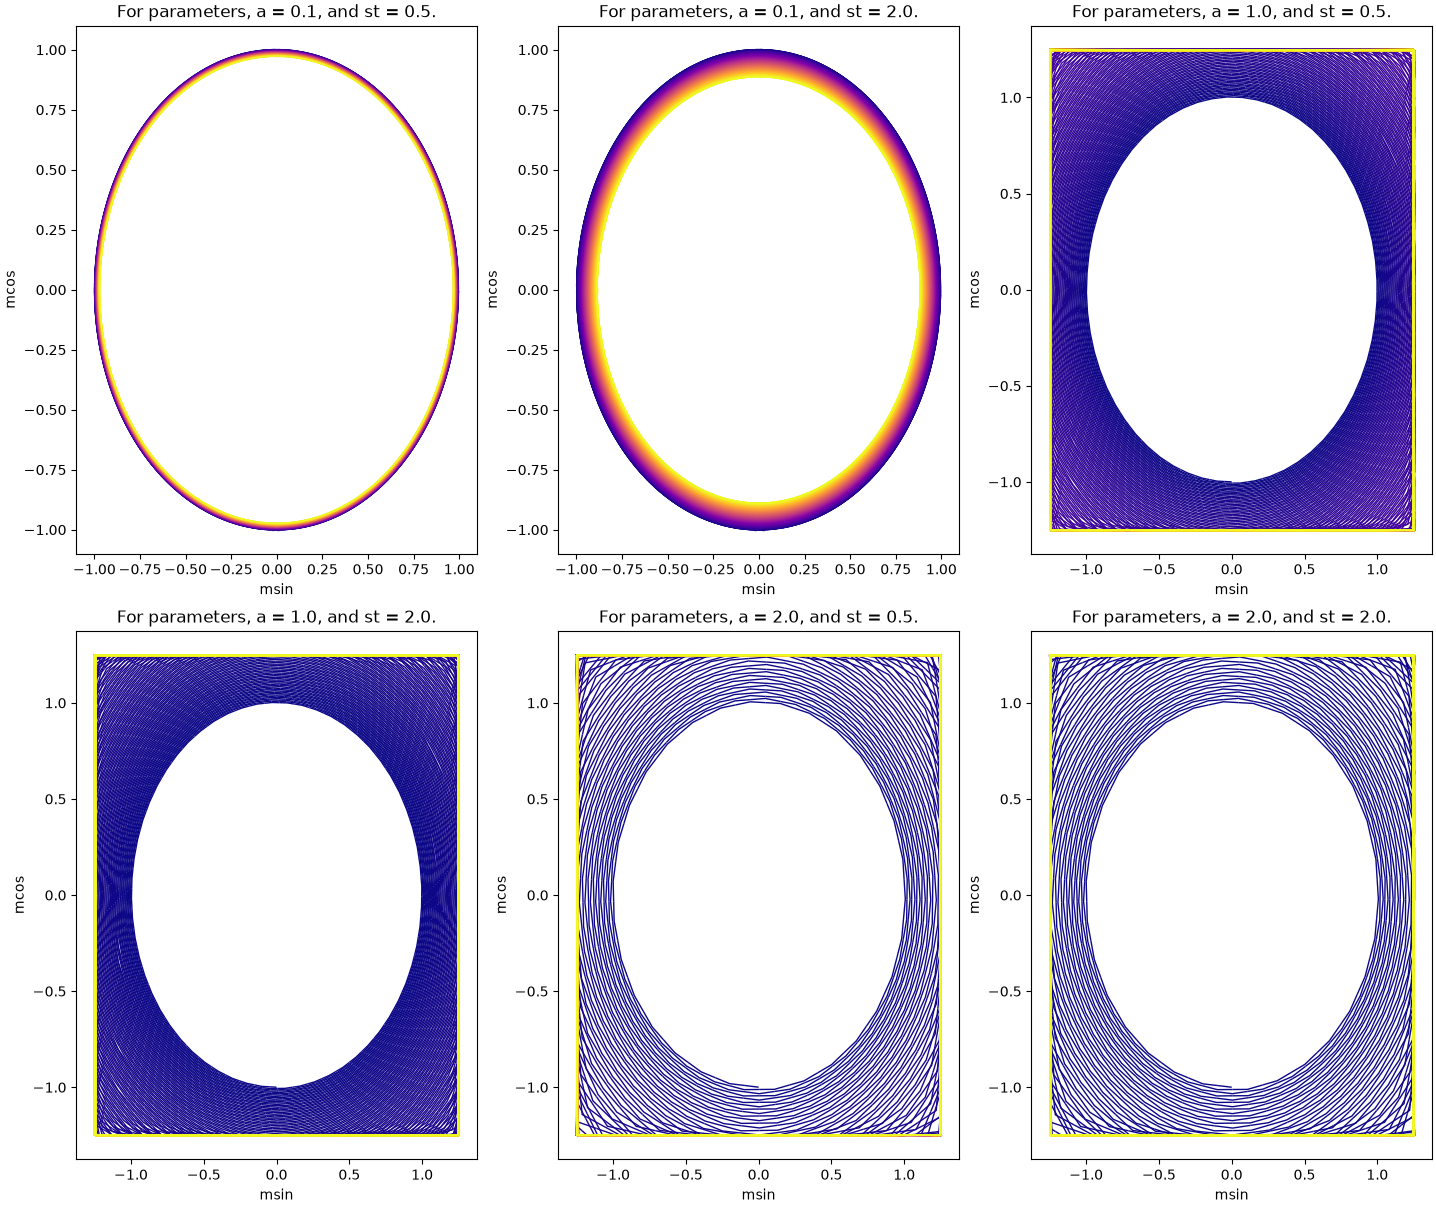
\includegraphics[width=1.0\textwidth]{images/harmonic_oscilator.png}
\caption{Plot of ODE's $f'(t) = g(t)$ and $g'(t) = -f(t)$, with $f(0) = 0$ and $g(0) = 1$. The parameter $rt$ denotes the simulation time. To indicate direction, the graph of the plot is colored over time, with purple at $t=0$ and yellow at $t=st$. The x axis is the output of the integrator that represents f, the y axis equally for g.}
\label{fig:figure1.1}
\end{figure}
\FloatBarrier




\problem{Differentiable convex functions PT1}
\label{problem-2}


\begin{lemma}
 \label{thm:eulers-identity}
 Let $V$ be a normed vector space viewed as a metric space and let $U \subseteq V$ be an open set of $V$ and $f \from U \to \Reals$ a continuous map. For $\alpha \in \mathbb{R}$, define
 \begin{align*}
   \Suba{f} = \{u \in U \mid f(u) < \alpha\}.
 \end{align*}
 Then $\Suba{f}$ is open and convex if $U$ and $f$ are convex.
\end{lemma}
\begin{proof}
 Firstly we show that $\Suba{f}$ is open in $V$. Since $f$ is continuous and $f$ is restricted on the open interval $(-\infty, \alpha)$ for any $u \in \Suba{f}$, we know that the pre-image of $f$ for $\Suba{f}$ is open in $U$. Since $U$ is a open in $V$ so must $\Suba{f}$ be an open in $V$.
  Secondly we show that $\Suba{f}$ is convex. Let $x,y \in U$ we know by definition that $x +_s y \in U$ for $s \in [0,1]$. With $f$ being convex:
 \begin{align*}
   f(sx + (1 - s)y) & \leq sf(x) + (1-s)f(y) & \\
    & \leq s\alpha  + (1-s)\alpha  = \alpha & (\forall z \in \Suba{f}. f(z) < \alpha )
 \end{align*}
 Thus, $x +_s y \in \Suba{f}$, making it convex.
\end{proof}


\problem{Differentiable convex functions PT2}
\label{problem-3}
a.
\begin{lemma}
 \label{thm:eulers-identity}
 The determinant of the Hessian of $g$ is equal to $4^2(3^2x_1^2y_2^2 - 1)$.
 \begin{align*}
   g(x) = x_1^4 + x_2^4 - 4x_1x_2
 \end{align*}
\end{lemma}
\begin{proof}
We first compute the Jacobian:
\begin{align*}
 \text{J}_g(x) &= \begin{pmatrix}
   4x_1^3 - 4x_2, \\
   4x_1^3 - 4x_1,
 \end{pmatrix}
\end{align*}
 then the Hessian:
\begin{align*}
 \text{Hess}_g(x) &= \begin{pmatrix}
   12x_1^2 & -4 \\
   -4 & 12x_2^2 \\
 \end{pmatrix}
\end{align*}
 The determinant follows:
\begin{align*}
 \det(\text{Hess}_g(x)) = 12^2x_1^2x_2^2 - 16 = 4^2(3^2x_1^2y_2^2 - 1)
\end{align*}
\end{proof}






\begin{lemma}
 \label{lemma:gradient_ineq_bound}
 Assuming $3^2x_1^2x_2^2 > 1$, the Hessian of $g$ is positive definite.
 \begin{align*}
   g(x) = x_1^4 + x_2^4 - 4x_1x_2
 \end{align*}
\end{lemma}
\begin{proof}
(b.) Using Sylvester's criterion; since $12x^2 > 0$ and
\begin{align*}
 \det(\text{Hess}_g(x)) &= 4^2(3^2x_1^2x_2^2 - 1) > 0 \\
     & 3^2x_1^2x_2^2 > 1
\end{align*}
$\text{Hess}_g(x)$ is positive definite.
\end{proof}


\begin{lemma}
 \label{thm:eulers-identity}
 Set $U \subset H_1$ given by
 \begin{align*}
   U = \{ x \in \Reals^2 \mid x_1 > 0 \text{ and } 3x_1x_2 >1 \}
 \end{align*}
 is open and convex.
\end{lemma}
\begin{proof}


 (c.) We want to define the continuous map $f \from H_1^2 \to \Reals$ such that:
 \begin{align*}
   \Subo{f} = \{x \in \Reals^2 \mid x_1 > 0 \text{ and } 3x_1x_2 &> 1 \}.\\
   3x_1x_2 &> 1  \\
   x_2 &> \frac{1}{3x_1}  \\
   0 &> \frac{1}{3x_1} - x_2
 \end{align*}
 Thus, using the restriction we define the map as: $f(x) = \frac{1}{3x_1} - x_2$.


 (d.) Firstly we show that $f$ is $0$-convex:
 \begin{align*}
   \langle \nabla f(x), y - x \rangle &\leq f(y) - f(x) - \alpha  \Vert  - y \Vert^2_2 &\\
   \frac{x_1 - y_1}{3x_1^2} - y_2  + x_2  &\leq \frac{1}{3y_1} - y_2 - \frac{1}{3x_1} + x_2  &(\text{see \cref{innerprod}})&\\
   \frac{x_1 - y_1}{3x_1^2} - y_2  + x_2  - \frac{1}{3y_1} + y_2 + \frac{1}{3x_1} - x_2  &\geq 0 &\\
   \frac{x_1 - y_1}{3x_1^2}  - \frac{1}{3y_1} + \frac{1}{3x_1}   &\geq 0 &\\
   \frac{x_1 - y_1 + 3x_1}{3x_1^2}  - \frac{1}{3y_1}   &\geq 0 &\\
   \frac{x_1 - y_1 + 3x_1 - 3x_1^2}{3x_1^2y_1}   &\geq 0 &\\
   \frac{(x_1 - y_1)^2}{3x_1^2y_1}   &\geq 0&
 \end{align*}
 This inequality holds because $x_1,y_1 > 0$, here follows the computation of the innerproduct.
 \begin{align} \label{innerprod}
   \langle \nabla f(x), y - x \rangle &= \langle  \begin{pmatrix}
     -\frac{1}{3x_1^2} \\
     -1
   \end{pmatrix}, (y - x) \rangle \\
   &= -\frac{y_1 - x_1}{3x_1^2} +  \frac{y_2  - x_2}{-1} \\
   &= \frac{x_1 - y_1}{3x_1^2} - y_2  + x_2
 \end{align}
  Then we show that the Hessian of $f$ is positive definite for all $x \in \Subo{f}$
 \begin{align*}
   \langle (\text{Hess}_f(x)-2aI)v, v\rangle \geq 0 \\
   \langle \begin{pmatrix}
     \frac{2}{3x_1^3} & 0 \\
     0 & 0
   \end{pmatrix} v, v\rangle \geq 0 \\
   \frac{2}{3v_1^3} * v_1 \geq 0 \\
   \frac{2}{3v_1^2} \geq 0
 \end{align*}
 This inequality holds for all directions $v \in \Reals^2$, hence $\Subo{f}$ is convex.
\end{proof}


\problem{Gradient flow}
\begin{lemma}
 \label{lemma:blabla}
 Let $U \subseteq \Reals^n$ is open, $f \in C^2(U)$, and $f$ has a local minimum $m \in U$. With some $\epsilon \in \Reals_{>0}$ and $f$ is $\alpha$-convex when restricted to $B_\epsilon(m)$. Then for all $x_0 \in B_\epsilon(m)$ the ODE $\gamma \from \Reals_{\geq 0} \to B_\epsilon(m)$ has a solution.
 \begin{align*}
   \gamma'(t) = -\nabla f(\gamma(t)) & & \gamma(0) = x_0
 \end{align*}
 Using Euclidean distance the following inequality holds for all $t \in \Reals_{\geq 0}$:
 \begin{align*}
   d(\gamma(t), m) \leq e^{-2at}d(x_0,m)
 \end{align*}
\end{lemma}
\begin{proof} We define the map $T(t) = \Vert\gamma(t) - m \Vert^2 = d(\gamma(t),m)^2$ and:
\begin{align*}
  T'(t) &= 2 \sum^n_{i=1}(\gamma_i(t) - m_i)  \gamma'_i(t) && (\text{chain rule}) \\
 &= 2 \langle \gamma(t) - m, \gamma'(t) \rangle && \\
 &= -2 \langle \gamma(t) - m, \nabla f(\gamma(t)) \rangle && (\text{substitude for } \gamma') \\
 &= -2 \langle \gamma(t) - m, \nabla f(\gamma(t)) - \nabla f(m) \rangle && (\nabla f(m) = 0)
\end{align*}


We know that $f$ is $\alpha$-convex, thus:
\begin{align*}
 2\alpha \Vert x - y \Vert ^2_2 &\leq \langle \nabla f(x) - \nabla f(y), x - y \rangle \\
 2\alpha \Vert \gamma(t) - m \Vert ^2_2 &\leq \langle \gamma(t) - m, \nabla f(\gamma(t)) - \nabla f(m) \rangle \\
 -4\alpha \Vert \gamma(t) - m \Vert ^2_2 &\geq -2\langle \gamma(t) - m, \nabla f(\gamma(t)) - \nabla f(m) \rangle = T'(t) \\
\end{align*}


Using Gr\"onwall's inequality: $f'(t) \leq w(t)f(t)$, we have $T'(t) \leq -4\alpha \Vert \gamma(t) - m \Vert ^2_2  \leq w(t)T(t)$, thus $-4 \alpha \leq w(t)$. Then the following inequality holds:
\begin{align*}
 d(\gamma(t),m)^2 &\leq T(0) e^{W(t)}  \\
 d(\gamma(t),m)^2 &\leq d(x_0, m)^2 e^{-4at}  \\
 d(\gamma(t),m) &\leq e^{-2at}d(x_0, m)
\end{align*}
\end{proof}




\problem{Convex optimisation on analog computers.}
Let $h \from \Reals \to \Reals$ given by $h(x) = x^2$. 
 
(a.) Its gradient is $\nabla h = 2x$. The ODE $\gamma'(t) = - \nabla h(\gamma(t)) = -2\gamma(t)$. We write the ODE using the fundamental theorem of calculus: $\gamma'(t) = h(0) -2 \int_0^t \gamma'(t)dt$. The circuit is just an integrator connected to itself. See the implementation of the circuit in appendix \cref{problem5code}.


(b.) See \cref{fig:hplot} for the plot of the gradient flow of $h$.


\begin{figure}[h]
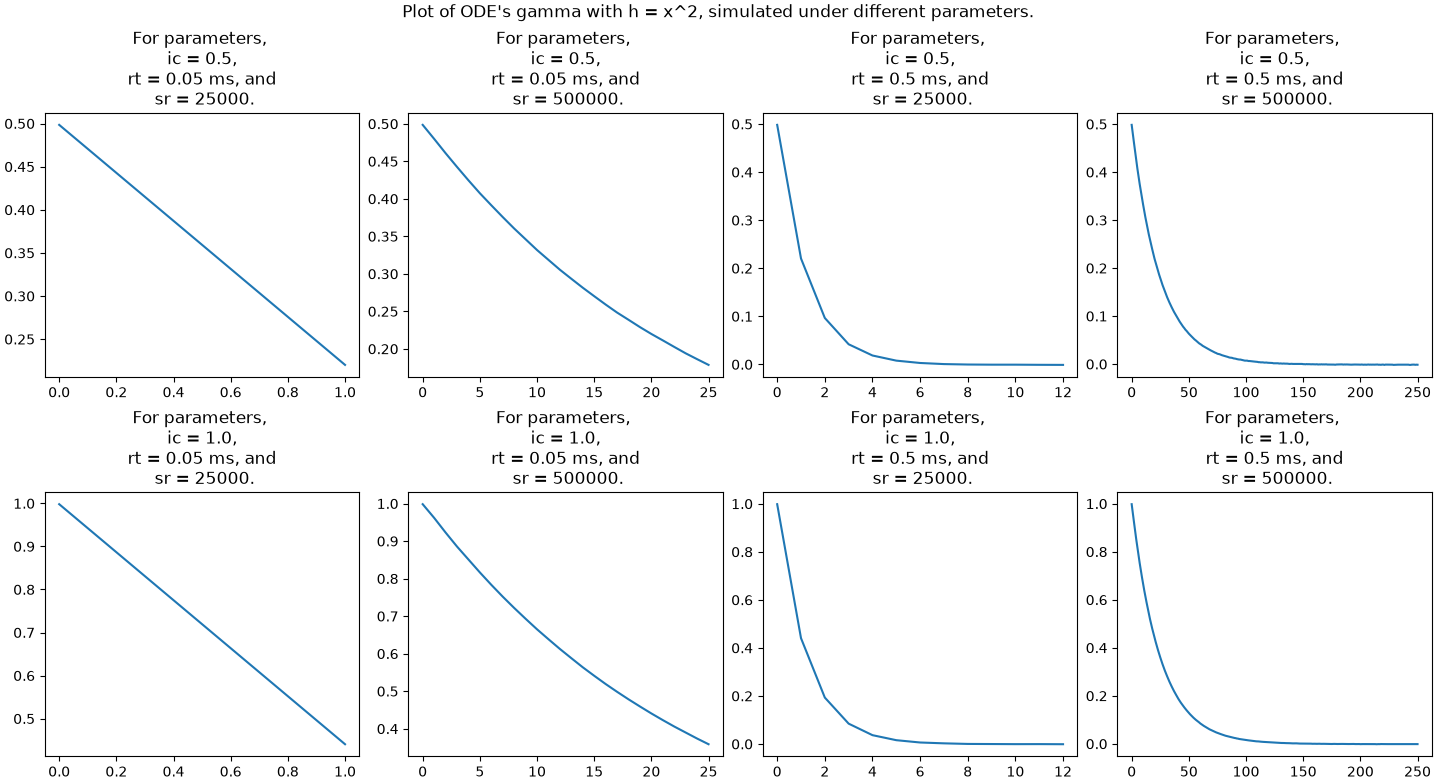
\includegraphics[width=1.0\textwidth]{images/h_plot.png}
\caption{Plot of the gradient flow of h(x). Parameters are titeld per plot, ic stands for initial condition, rt stands for simulation time, and, sr stands for sample rate. Time on the x axis and the output value of the integrator on the y axis.}
\label{fig:hplot}
\end{figure}
\FloatBarrier


(c.) From lemma \ref{lemma:blabla} we know that the distance to the minimum is bounded by $e^{-2\alpha t}d(x_0, m)$ for all $x_0 \in B_\epsilon(m)$. Which is equally depicted in the plots above, there is an exponential decay from the initial value towards the minimum of $f$.


(d.) The longer the simulation runs the closer the approximation reaches the minimum. A higher sample rate smoothens the graph of the plot, which is shown by for example the first two plots; the higher sample rate smoothens the graph into a convex bent.


\problem{Symbolic computation library}
See attached python library (directory "analog\_optimizer" in the repository) and an example program (example.py in the root directory). The gradient is implemented through the classmethod \_gradient(). Furthermore the parser of the expression tree into a circuit is implemented in parser.py. $R_>0Mod$ is implemented in r0mod.py and has strong convexity in the ExpressionConvex class in expression.py.


\problem{Example}
The example implements the function $g$ from problem \cref{problem-3} and its gradient.


\begin{figure}[h]
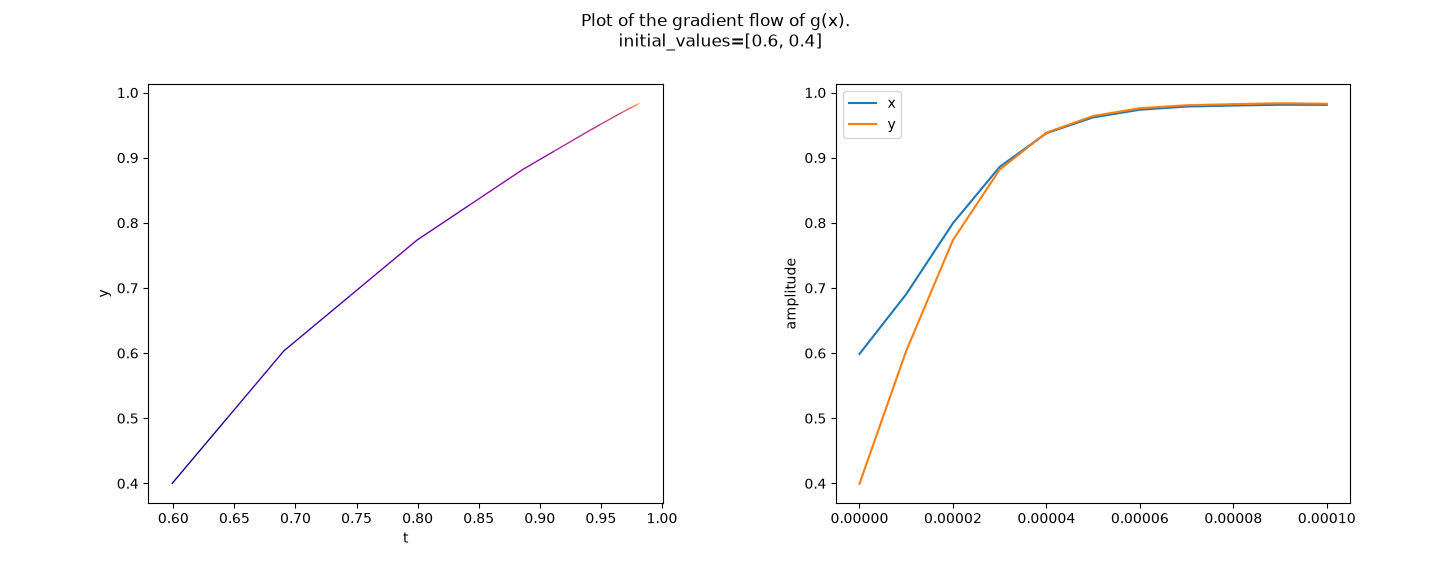
\includegraphics[width=1.0\textwidth]{images/gradient_flow_of_g.png}
\caption{Plot of the gradient flow of g(x), the circuit was generated using the ParseTree class in parser.py. Initial conditions where 0.4 and 0.6. At sample rate 100.000 Hz and the simulation time of 100 microseconds.}
\label{fig:gradient_flow}
\end{figure}
\FloatBarrier




\printbibliography{}

\appendix

\section{Code for problem 5} \label{problem5code}
\lstset{basicstyle=\small, keywordstyle=\bfseries}
\begin{lstlisting}[language=Python]
import asyncio
import numpy as np
from matplotlib import pyplot as plt
from pybrid.lucipy import Circuit, LUCIDAC, time_series
luci = LUCIDAC("tcp://192.168.1.5:5732")
ic_values = [ 0.5,  1.0 ]
rt_values = [ 0.05,  0.5 ]
sr_values = [ 25000, 500_000 ]
iter_values = [ (ic, rt, sr) for ic in ic_values  \
                             for rt in rt_values for sr in sr_values ]
fig, axs = plt.subplots(2,4,layout='constrained'  )
for i, ax in enumerate(axs.flat):
   (ic, rt, sr) = iter_values[i]
   print(ic, rt, sr)
   l = luci.create_circuit()
   m_gamma = l.int(ic=-ic)
   l.probe(m_gamma, adc_channel=0)
   l.connect(m_gamma, m_gamma, weight=2.0)
   luci.set_daq(num_channels=1, sample_rate=sr)
   luci.set_run(op_time=int(rt * 1_000_000))
   run = luci.run()
   t = np.arange(len(run.data[0]))
   ax.plot(t, run.data[0], label="gamma")
   ax.set_title(f"For parameters, \n ic = {ic}, \n rt = {rt} ms, and \n sr = {sr}.")
fig.suptitle("Plot of ODE's gamma with h = x^2, simulated under different parameters.")
plt.show()
\end{lstlisting}


\end{document}



